%% Use the "normalphoto" option if you want a normal photo instead of cropped to a circle
% \documentclass[10pt,a4paper,normalphoto]{altacv}

\documentclass[10pt,a4paper,ragged2e,withhyper]{altacv}
%% AltaCV uses the fontawesome5 and simpleicons packages.
%% See http://texdoc.net/pkg/fontawesome5 and http://texdoc.net/pkg/simpleicons for full list of symbols.

% Change the page layout if you need to
\geometry{left=1.25cm,right=1.25cm,top=1.5cm,bottom=1.5cm,columnsep=1.2cm}

% The paracol package lets you typeset columns of text in parallel
\usepackage{paracol}


% Change the font if you want to, depending on whether
% you're using pdflatex or xelatex/lualatex
% WHEN COMPILING WITH XELATEX PLEASE USE
% xelatex -shell-escape -output-driver="xdvipdfmx -z 0" mmayer.tex
\iftutex
  % If using xelatex or lualatex:
  \setmainfont{Lato}
\else
  % If using pdflatex:
  \usepackage[default]{lato}
\fi

% Change the colours if you want to
\definecolor{AlmostBlack}{HTML}{0D0D0D}
\definecolor{VividPurple}{HTML}{3E0097}
\definecolor{SlateGrey}{HTML}{2E2E2E}
\definecolor{LightGrey}{HTML}{666666}
% \colorlet{name}{black}
\colorlet{tagline}{SlateGrey}
\colorlet{heading}{AlmostBlack}
\colorlet{headingrule}{AlmostBlack}
% \colorlet{subheading}{PastelRed}
\colorlet{accent}{AlmostBlack}
\colorlet{emphasis}{SlateGrey}
\colorlet{body}{LightGrey}



\renewcommand{\cvItemMarker}{{\small\textbullet}}
\renewcommand{\cvRatingMarker}{\faCircle}
\renewcommand{\taglinefont}{\LARGE\bfseries}
\usepackage{tikz}
\newcommand{\maindivider}{%
  \noindent
  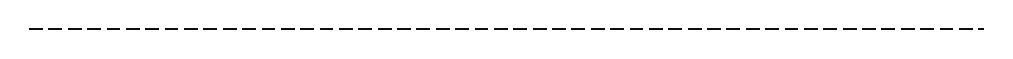
\begin{tikzpicture}
    \draw[headingrule, line width=1pt, dash pattern=on 5pt off 2pt] (0,0) -- (\linewidth,0);
  \end{tikzpicture}\par\vspace{0.3em}%
}
\input{pubs-num.tex}

%% sample.bib contains your publications
\addbibresource{sample.bib}

\begin{document}
\name{Adrien Sourdille}
\tagline{Analytics Engineer}
% Cropped to square from https://en.wikipedia.org/wiki/Marissa_Mayer#/media/File:Marissa_Mayer_May_2014_(cropped).jpg, CC-BY 2.0
% \photoL{2cm}{images/Yacht_High,images/Suitcase_High}
\personalinfo{%
  \email{adriensourdille99@gmail.com}
  \phone{+33 (0)7 85 76 66 85}
  \location{UK, London}
  \linkedin{adrien-sourdille}
  \github{AdrienSourdilleTIL} 
}

\makecvheader

%% Depending on your tastes, you may want to make fonts of itemize environments slightly smaller
\AtBeginEnvironment{itemize}{\small}

%% Set the left/right column width ratio to 6:4.
\columnratio{0.6}

% Start a 2-column paracol. Both the left and right columns will automatically
% break across pages if things get too long.
\begin{paracol}{2}

\cvsection{Relevant Experience}

\cvevent{Consulting Data Analyst \& Data Engineer}{The Information Lab}{February 2023 -- Ongoing}{London, UK}
\begin{itemize}
\item Undertook a 4 month intensive data analytics training program with one of the UK's top data analytics consultancies, followed by 3 years of consulting work across various industries. This period involved developing advanced technical skills in Snowflake, GCP, Azure, dbt, Tableau, and Alteryx. Also honed were skills in managing clients and stakeholders, along with cultivating a high standard in presentation abilities.
\end{itemize}

\maindivider

\cvevent{Data Engineer}{Virgin Media O2}{August 2025-Ongoing}{London, UK}

\begin{itemize}
\item Designed and developed a pioneering pipeline linking network performance data with customer metrics, enabling end-to-end measurement of a £700m infrastructure investment’s impact on performance, satisfaction, churn, and revenue.
\end{itemize}
\vspace{0.1cm} % Adjust the space as needed
\cvtag{GCP}
\cvtag{SQL}
\cvtag{dbt}
\cvtag{Jira}
\cvtag{Gitlab}

\divider

\cvevent{Data Engineer}{Prêt a Manger}{November 2024 -- June 2025}{London, UK}
\begin{itemize}
\item Engineered robust ETL pipelines in Snowflake to process complex live order data from hundreds of shops across 5 countries. Developed custom SQL and JSON unnesting scripts to transform messy transactional data into structured insights on revenue, stock, tax, and waste.
\item Led a core component of the company’s migration from a legacy SQL Server system to Snowflake, contributing to multi-million-pound savings in infrastructure and licensing costs.
\item Re-engineered the broken “Active Till” report to identify underused and overused tills, automating its data pipeline and reducing reporting time by over 80%.
\end{itemize}
\vspace{0.1cm}
\cvtag{Snowflake}
\cvtag{SQL}
\cvtag{Github}
\cvtag{Javascript}
\cvtag{Jira}
\cvtag{GCP}
\cvtag{Azure}

\divider

\cvevent{Data Analyst}{BAE Systems}{June 2023 -- June 2024}{London, UK}
\begin{itemize}
\item Scoped, built, and automated a key financial report to track the company’s R\&D budget and spending using chained Alteryx apps, and delivered an interactive Tableau dashboard securely accessible on Tableau Server.
\item Built a Tableau dashboard to identify multimillion-pound technology investments, highlighting new opportunities and tracking the progress of prior initiatives.
\end{itemize}
\vspace{0.1cm} % Adjust the space as needed
\cvtag{Tableau Suite}
\cvtag{Alteryx Suite}
\cvtag{Jira}

\switchcolumn

\cvsection{Education}

\cvevent{Master of Geographic Data Science}{London School of Economics (LSE)}{2021 -- 2022}{London, UK}
\begin{itemize}
\item Studied reinforcement learning, environmental economics, GIS and spatial data analysis
\item Answered causal research questions and developed rigorous scientific methods
\end{itemize}


\cvsection{Personal Statement}


{\color{SlateGrey} \itshape \normalsize
Analytics Engineer with three years of consulting experience designing and delivering client-focused data solutions across a wide range of industries. Strong emphasis on collaboration, client management, and stakeholder engagement, combined with solid technical expertise in Snowflake, dbt, Tableau, and Alteryx. Particularly motivated by using data expertise to drive environmental sustainability and support the energy transition.
}

\cvsection{Certifications}

\begin{minipage}[c]{0.08\linewidth}
  
\includegraphics[width=\linewidth]{images/tableau-certified-data-analyst.png}
\end{minipage}%
\hspace{0.5em}%
\begin{minipage}[c]{0.9\linewidth}
  \textbf{Tableau Data Analyst}
\end{minipage}

\vspace{0.5em}

\begin{minipage}[c]{0.08\linewidth}
  
\includegraphics[width=\linewidth]{images/Snowpro-core.png}
\end{minipage}%
\hspace{0.5em}%
\begin{minipage}[c]{0.9\linewidth}
  \textbf{SnowPro Core}
\end{minipage}

\vspace{0.5em}

\begin{minipage}[c]{0.08\linewidth}
  
\includegraphics[width=\linewidth]{images/alteryx-designer-advanced-certification.png}
\end{minipage}%
\hspace{0.5em}%
\begin{minipage}[c]{0.9\linewidth}
  \textbf{Alteryx Designer Advanced}
\end{minipage}


\cvsection{Stack}

% Don't overuse these \cvtag boxes — they're just eye-candies and not essential. If something doesn't fit on a single line, it probably works better as part of an itemized list (probably inlined itemized list), or just as a comma-separated list of strengths.

% The `ragged2e` document class option might cause automatic linebreaks between \cvtag to fail.
% Either remove the ragged2e option; or 
% add \LaTeXraggedright in the paragraph for these \cvtag
\cvtag{Tableau Suite}
\cvtag{Alteryx Suite}
\cvtag{SQL}
\cvtag{dbt}
\cvtag{Javascript}
\cvtag{Python}
\cvtag{Jira}
\cvtag{Github}
\cvtag{Gitlab}
\cvtag{Snowflake}
\cvtag{GCP}
\cvtag{Azure}

\cvsection{Languages}

\cvskill{English}{5}
% \divider

\cvskill{French}{5}
% \divider

\cvskill{Italian}{3.5} %% supports X.5 values.

\vspace{0.5cm}

\href{https://adriensourdilletil.github.io/AdrienSourdillePortfolio/}{\faBriefcase\ Visit my Portfolio Website}

\vspace{0.25cm} % Adjust the space as needed

\href{https://public.tableau.com/app/profile/adrien.sourdille4093/vizzes}{\faHome\ Visit my Tableau Public}


\end{paracol}

\end{document}